\chapter{Úvod}
V súčasti sa pre ľudí stávajú vnútorné prostredia budov miestom, kde trávia najviac času, približne 90\,\%. Je to dôsledok modernej doby, kde sa väčšina času trávi v kanceláriách, školách alebo obytných priestoroch. V týchto priestoroch dýchame vnútorné ovzdušie, ktoré je ovplyvnené kvalitou vonkajšieho vzduchu. Dôvodom tohto ovplyvňovania je vetranie, ktoré privádza vonkajší čerství vzduch do budov a odvádza vzduch obsahujúci znečisťujúce látky von z budov. Vnímanie kvality vnútorného ovzdušia je subjektívne hodnotenie, ktoré sa môže skladať z rôznych faktorov ako kvalita vonkajšieho vzduchu, objem vzduchu pripadajúceho na jednu osobu v miestnosti, alebo aj ako množstvo znečisťujúcich látok, kde zdrojom môžu byť obyvatelia a ich metabolizmus alebo samotný materiál, s ktorého je budova postavená. 

Mnoho budov má riadenú výmenu vzduchu podľa dopredu daného časového harmonogramu a počtu očakávaných ľudí vo vybraných priestoroch. V prípade zvýšenia počtu ľudí nad neočakávanú hranicu môže dôjsť k nedostatočnej výmene vzduchu a postupnému zhoršovaniu kvality vnútorného prostredia. Druhým prípadom je, zbytočné privádzanie veľkého objemu čerstvého vzduchu do priestorov, kde sa nachádza výrazne menej osôb ako bolo plánované.

Tendenciou znižovania energetickej náročnosti budov dochádza k používaniu nových materiálov, ktoré eliminujú infiltráciu vonkajšieho vzduchu. Infiltráciou sa rozumie prirodzené vetranie netesnosťami pomocou vonkajšej obálky budovy (napr. netesné škáry okenných a dverných otvorov). Moderné technológie a materiály obmedzujú túto infiltráciu tak výrazne, že bez riadenej ventilácie alebo mechanického otvárania okien dochádza k rýchlemu nárastu nežiadúcich látok vo vzduchu, čo môže spôsobiť zdravotné problémy. 

Celková kvalita vnútorného ovzdušia ovplyvňuje naše fyzické zdravie a duševnú pohodu.  Zdravotné problémy môže spôsobiť zlá kvalita vnútorného ovzdušia, teplota alebo vlhkosť. Nevyhovujúca teplota a vlhkosť spolu s nedostatočným vetraním môžu spôsobiť rast pliesní a ďalších alergénov. 

Podľa vyhlášky č. 20/2012 Sb. Českej republiky o technických požiadavkách na stavby je ukazovateľom kvality vnútorného prostredia koncentrácia oxidu uhličitého, ktorá by nemala presiahnuť hranicu 1500\,ppm. Po prekročení tejto hodnoty môže dochádzať k únave, bolestiam hlavy, hrdla alebo k vzniku astmy, pričom vysoká koncentrácia $CO_2$ môže mať na ľudí rozdielne účinky. 

Koncentrácia oxidu uhličitého vo vnútornom prostredí závisí najmä od množstva a kvality privádzaného čerstvého vzduchu a od počtu osôb nachádzajúcich sa v danom prostredí. Množstvo oxidu uhličitého, ktoré osoby vyprodukujú závisí od ich činnosti a hmotnosti. Čím je vykonávaná fyzicky náročnejšia práca, tým sa u ľudí spaľuje viacej glukózy, pričom sa vytvára väčšie množstvo oxidu uhličitého a jeho koncentrácia rastie rýchlejšie. Koncentráciu ovplyvňujú aj rastliny, ktoré fotosyntézou premieňajú oxid uhličitý na kyslík.

%Existujú softwérové riešenia, ktoré umožnia vypočítať
V dnešnej modernej dobe sú ventilačné systémy uspôsobené na určitý počet osôb v miestnosti, prípadne na časový harmonogram. Takýto spôsob však nie je efektívny v prípade nečakaného zvýšenia počtu osôb v miestnosti alebo v opačnom prípade, kedy z nejakých príčin (dovolenka, chrípka) sa na pracovisku vyskytuje podstatne menej osôb ako obyčajne. Niektoré budovy z rozličných dôvodov nemôžu mať ventilačné systémy a musia vetranie vykonávať mechanicky (ručné otvorenie okna). Informáciu o tom ako dlho a kedy majú vetrať je len subjektívny pohľad danej osoby. V týchto budovách môžu byť umiestnené meracie prístroje, ktoré  umožňujú merať, prípadne aj signalizovať koncentráciu oxidu uhličitého. Neumožňujú však predpovedať ako dlho by toto vetranie malo prebiehať v závislosti na počte osôb a rozlohe miestnosti. 

Cieľom práce je tak vybrať vhodné senzory na meranie oxidu uhličitého vo vnútri budov a na základe vykonaných meraní stanoviť závislosť koncentrácie oxidu uhličitého na nameraných veličinách. Na základe stanovenej závislosti vytvoriť atribúty pre strojové učenie a vytvoriť model pre detekciu otvorenia okna.

%ako spravne vetrat a treba sa tym zaoberat

\chapter{Kvalita ovzdušia}
Vo všeobecnosti závisí kvalita vnútorného ovzdušia na kvalite vonkajšieho ovzdušia, pretože vetraním privádzame do budov vonkajší vzduch. Na jednej strane sa vetraním odvádzajú škodliviny vzniknuté v budove a na druhej strane sa privádzajú škodliviny z vonkajšieho ovzdušia do budovy.

Mieru kvality ovzdušia upravuje zákon a potom ďalej špecifikujú vyhlášky, ktoré sú špecifické pre danú krajinu. Pre Slovenskú republiku je to zákon č. 137/2010 Z. z. a pre Českú republiku zákon č. 201/2012 Sb.

\section{Vonkajšie ovzdušie}
Kvalitu vonkajšieho ovzdušia určuje obsah znečisťujúcich látok vo vonkajšom ovzduší. Znečistenie spôsobujú hlavne rôzne druhy spaľovacích procesov, ktoré je možné pozorovať v priemysle, výrobe energií a doprave. Medzi hlavné znečisťujúce látky v Českej republike patria tuhé látky (oxid siričitý, oxidy dusíka, oxid uhoľnatý, polyaromatické uhľovodíky, prchavé organické látky a amoniak) \cite{KvalitaVzduchu}. 

Je dokázané, že ovzdušie obsahujúce znečisťujúce látky môže mať významné zdravotné dopady v podobe výskytu rôznych chorôb a problémov, prípadne zhoršenie existujúcich príznakov, ktoré sú spojené s dýchacími cestami \cite{VonkajsieOvzdusie}. 

\section{Vnútorné ovzdušie}
V prostredí, ktoré sa nachádza vo vnútri budov trávime najviac času, približne 90\,\%. Toto prostredie má významný vplyv na naše fyzické zdravie. Problém nastáva s kvalitou vnútorného ovzdušia, ktorá je daná kombináciou vnútorných zdrojov a prenikaním škodlivín z vonkajšieho ovzdušia. Dominantný význam majú faktory prostredia, ktoré v budovách zapríčiňujú rast pliesní, alergénov a predstavujú zdravotné riziko pre osoby v týchto priestoroch \cite{VnutorneOvzdusie}.

Kvalitu vnútorného prostredia ovplyvňujú nasledujúce faktory \cite{IndoorAirQualityAndHealt}:
\begin{itemize}
    \item fyzikálne - prúdenie vzduchu, hluk, teplota a vlhkosť,
    \item chemické - oxid uhličitý, uhoľnatý a dusičitý, anorganické a organické škodliviny, prchavé organické látky, azbest alebo fajčenie,
    \item biologické - baktérie, vírusy, plesne, roztoče prach a domáce zvieratá.
\end{itemize}

Hodnotenie kvality vnútorného prostredia je subjektívne hodnotenie a je závislé na rozličných faktoroch \cite{KvalitaVnutornehoProstredia}:
\begin{itemize}
    \item kvalite vonkajšieho ovzdušia,
    \item objemu vzduchu pripadajúceho na osobu v miestnosti,
    \item výmene vzduchu,
    \item množstve znečisťujúcich látok v ovzduší, kde týmto zdrojom môžu byť:
    \begin{itemize}
        \item ľudia, zvieratá, rastliny a ich metabolizmus,
        \item aktivity ľudí a zvierat,
        \item stavebný materiál,
        \item upratovanie, čistenie a údržba budov.
    \end{itemize}
\end{itemize}

\section{Syndróm chorých budov}
Syndróm chorých budov (SBS -- Sick Building Syndrom) je pojem používaný pre nešpecifikované symptómy súvisiace s pobytom v budovách. Ľudia vo vnútri budov sa sťažujú na symptómy ako: podráždenie očí, nosu, krku, bolesti hlavy, krku, únava, alergie -- prípadne prechod do astmy, suchá pokožka, horúčky alebo kašeľ \cite{SickBuildingSyndrome}.

Jednotliví ľudia sa môžu sťažovať na rozdielne symptómy. Ak je počet sťažujúcich sa ľudí väčší než 20\,\% po dobu aspoň dvoch týždňov, môžeme budovu označiť za chorú \cite{SickBuildingSyndrome}.

Príčiny vzniku SBS môžeme hľadať v nových konštrukciách budov, zatepľovaní budov alebo v používaní plastových okien. Tieto nové konštrukcie a materiály šetria energiu a umožňujú menšiu infiltráciu vonkajšieho vzduchu. Okrem samotných budov a materiálov, z ktorých sú zhotovené, prispievajú k znečisťovaniu vnútorného prostredia technológie (počítače, tlačiarne), nábytok, koberce, či samotné mechanické vetranie, ktoré je potrebné pravidelne kontrolovať a čistiť \cite{SickBuildingSyndrome}.

Výskumníci z National Institute for Occupational Safety and Health (NIOSH) vykonali výskum v USA v roku 1983, kde bolo otestovaných 203 budov, z ktorého vyplýva, že hlavnou príčinou SBS je nedostatočné vetranie, ktoré tvori skoro polovicu (48\,\%) celkového znečistenia budov \cite{SickBuildingSyndrome} ako je možné vidieť v tabuľke \ref{nioshTable}.

\begin{table}[H]
\centering
\label{nioshTable}
\begin{tabular}{|l|c|c|}
\hline
\textbf{Pôvod znečistenia} & \textbf{Počet výskytov} & \textbf{\begin{tabular}[c]{@{}c@{}}Výskyt\\ {[}\%{]}\end{tabular}} \\ \hline
Nedostatočné vetranie & 98 & 48 \\ \hline
Kontaminácia (vnútorná) & 36 & 18 \\ \hline
Kontaminácia (vonkajšia) & 21 & 10 \\ \hline
Neznáme & 19 & 9 \\ \hline
Vlhkosť & 9 & 4 \\ \hline
Kontaminácia (konštrukcia budovy) & 7 & 3 \\ \hline
Mikrobiologická kontaminácia & 6 & 3 \\ \hline
Cigaretový dym & 4 & 2 \\ \hline
Hluk, osvetlenie & 2 & 1 \\ \hline
Svrab & 1 & 2 \\ \hline
\end{tabular}
\caption{Výsledky výskumu NIOSH \cite{SickBuildingSyndrome}}
\end{table}

\section{Oxid uhličitý $CO_2$}
Oxid uhličitý, tiež nazývaný aj kysličník uhličitý, je stály, bezfarebný, nehorľavý, atmosferický plyn bez chuti a zápachu. Pri väčšej koncentrácií môže mať v ústach kyslú chuť s ľahko štipľavým zápachom. Jeho koncentrácia v ovzduší sa pohybuje v rozmedzí 350--400\,ppm. V okolí priemyselných zón a dopravných tepien môže byť koncentrácia vyššia, okolo 450\,ppm, prípadne aj viac. Oxid uhličitý sa skladá z jedného atómu uhlíka a dvoch atómov kyslíka. Oxid uhličitý je často označovaný svojou rovnicou $CO_2$ a je približne 1,5-krát ťažší než vzduch \cite{ucebnicaChemie}.

Koncentrácia oxidu uhličitého sa najčastejšie udáva v týchto jednotkách s nasledujúcim prevodom \cite{niosh}: 

%\ = \ 0,0001\,\%
\begin{equation}
    1\,ppm\ = \ 0,0001\,\% \ = \ 1.8\,\frac{mg}{m^3}
\end{equation}

Jednotka $ppm$ označuje \textit{parts per milion}, čo značí jednu časticu látky na každých 999\,999 iných častíc.

Podľa vyhlášky pre Českú republiku slúži oxid uhličitý ako ukazovateľ kvality vnútorného prostredia a jeho koncentrácia vo vnútornom ovzduší nesmie prekročiť hodnotu 1500\,ppm. Vyhláška ďalej definuje minimálne množstvo vymieňaného vonkajšieho vzduchu $25\,m^3/h $ a minimálnu intenzitu vetrania $0,5\,l/h$ pre obytnú miestnosť \cite{VyhlaskaKvalitaVnutornehoOvzdusiaCO}. 

\subsection{Pettenkoferovo kritérium}
Max Joseph von Pettenkofer preukázal, že hlavnými produktami látkovej výmeny je oxid uhličitý a vodná para. Meraním množstva $CO_2$ vo vydýchanom vzduchu zistil, že produkcia $CO_2$ závisí na fyzickej aktivite. Osoba v bdelom stave produkuje približne 16\,l/h $CO_2$. Ďalej zistil, že koncentrácia $CO_2$ informuje o kvalite vnútorného prostredia a stanovil maximálne prípustné množstvo $CO_2$ na 1000\,ppm. Z čoho vyplýva dávka čerstvého vzduchu pre jednu dospelú osobu na 25\,$m^3/h$ \cite{PettenkoferovoKriterium}.

\subsection{Produkcia $CO_2$ a $CO$}
Oxid uhličitý vzniká hlavne pri spaľovacích procesoch reakciou uhlíka a kyslíka alebo ako produkt metabolizmu živých organizmov. Prirodzeným procesom vo voľnej prírode vzniká: únikom zo sopky, hnitím, kvasením, dýchaním alebo dôsledkom ľudskej činnosti (antropogénne $CO_2$) \cite{AtmosferaAKlima}.

Antropogénne $CO_2$ sa vytvára predovšetkým počas spaľovania fosílnych a organických palív. Spaľovanie palív je dej, pri ktorom sa zlučujú prvky, ktoré sa nachádzajú v palive s kyslíkom, ktorý je súčasťou atmosferického vzduchu. Počas dokonalého spaľovacieho procesu sa uhlík v palive zlúči s kyslíkom vo vzduchu a vznikne oxid uhličitý podľa nasledujúcej rovnice \cite{Hemoglobin}:

\begin{equation}
    C + O_2 \longrightarrow CO_2    
\end{equation}

Oxid uhoľnatý ($CO$) vzniká pri nedokonalom spaľovaní fosílnych palív, pri požiari v uzavretých priestoroch alebo sa nachádza vo výfukových plynoch. Pre človeka je $CO$ toxický a vo vyšších koncentráciách môže spôsobiť až smrť. Dôvodom je, že $CO$ sa viaže v krvi na hemoglobín 250--300-krát pevnejšie než kyslík, a tak znemožňuje hemoglobínu v transporte kyslíka z pľúc do tkanív \cite{Hemoglobin}. $CO$ vzniká nasledujúcim spôsobom:
\begin{equation}
    2\ C + O_2 \longrightarrow 2\ CO
\end{equation}

Hlavným zdrojom $CO_2$ vo vnútri budov je respirácia. Respirácia je proces získavania energie rozložením cukrov na bunkovej úrovni. Proces respirácie môžeme nazvať dýchaním, ak sa jedná o ľudí, prípadne fotosyntézou, ak sa jedná o rastliny. Reakciou glukózy a kyslíka pri dýchaní vzniknú produkty: oxid uhličitý, voda a ATP (adenozín trifosfát -- energia) nasledujúcou reakciou \cite{PhotosynthesisRespiracia}:
\begin{equation}
    C_6 H_{12} O_6 + 6\ O_2 \longrightarrow 6\ H_2O + 6\ CO_2
\end{equation}

\subsection{Využitie $CO_2$}
Rastliny okrem respirácie umožňujú aj fotosyntézu. Fotosyntéza je opačný dej ako respirácia a na vstupe tohto procesu je: voda, oxid uhličitý, chlorofyl a energia (svetlo). Produktom fotosyntézy je kyslík a glukóza, ktoré vzniknú nasledujúcou reakciou \cite{PhotosynthesisRespiracia}:
\begin{equation}
     6\ H_2O + 6\ CO_2 \longrightarrow C_6 H_{12} O_6 + 6\ O_2
\end{equation}

\noindent Okrem procesu fotosyntézy je možné $CO_2$ využiť v bežnom živote a to pri \cite{VyuzitieCO2}:
\begin{itemize}
    \item extrakcií chmeľu pre použitie v pivovarníctve
    \item odstraňovaní kofeínu z kávy a čaju
    \item výrobe sýtených nápojov
    \item ochrane výrobkov pred pôsobením kyslíka ako ochranná atmosféra
    \item napĺňaní sprejov, kde nahradzuje plyny, ktoré poškodzujú ozónovú vrstvu
    \item napĺňaní hasiacich prístrojov suchým ľadom
\end{itemize}

\subsection{Vplyv $CO_2$ na zdravie ľudí}
Obsah oxidu uhličitého v atmosférickom vzduchu je nízky a nepredstavuje zdravotné problémy vo vonkajšom prostredí. Problémom sú uzavreté miestnosti, kde koncentrácia $CO_2$ môže rýchlo narásť, čo vedie k zvýšenej únave a k zníženej produktivite osôb nachádzajúcich sa v daných priestoroch. Taktiež sa môžu vyskytnúť bolesti hlavy, respiračné problémy a ochorenia dýchacích ciest. Spomenuté zdravotné problémy môžeme pozorovať v priestoroch, ktoré sú nedostatočne vetrané, alebo v priestoroch s väčším počtom ľudí (divadlá, auly, školy, kancelárie) \cite{VplyvOxiduUhlicitehoNaLudskyOrganizmus}.

\begin{table}[H]
\centering
\label{ucinkyCO2}
\begin{tabular}{|c|l|}
\hline
\textbf{Koncentrácia $CO_2$} & \multicolumn{1}{c|}{\textbf{Vplyv $CO_2$ na ľudský organizmus}} \\ \hline
cca 350\,ppm & úroveň vonkajšieho prostredia \\ \hline
do 1000\,ppm & doporučená úroveň $CO_2$ vo vnútorných priestoroch \\ \hline
1200--1500\,ppm & doporučená maximálna úroveň $CO_2$ vo vnútorných priestoroch \\ \hline
1000--2000\,ppm & nastávajú príznaky únavy a znižovanie koncentrácie \\ \hline
2000--5000\,ppm & nastávajú možné bolesti hlavy \\ \hline
$<= \ 5000$\,ppm & maximálna bezpečná koncentrácia bez zdravotných rizík \\ \hline
\textgreater \ 5000\,ppm & nevoľnosť a zvýšený tep \\ \hline
\textgreater \ 15000\,ppm & dýchacie problémy \\ \hline
\textgreater \ 40000\,ppm & možná strata vedomia \\ \hline
\end{tabular}
\caption{Vplyv $CO_2$ na ľudský organizmus \cite{VplyvOxiduUhlicitehoNaLudskyOrganizmus}}
\end{table}

Jednotlivé účinky na ľudský organizmus záležia od koncentrácie $CO_2$ vo vzduchu v daných priestoroch a môžu sa líšiť v závislosti na jednotlivých osobách. Doporučená maximálna úroveň $CO_2$ je stanovená v rozsahu 1200--1500\,ppm\cite{VyhlaskaKvalitaVnutornehoOvzdusiaCO} a jednotlivé účinky sa opierajú o koncentráciu $CO_2$ vo vzduchu, ktoré sú uvedené v tabuľke \ref{ucinkyCO2}. Za bezpečnú hranicu koncentrácie $CO_2$ sa považuje hodnota 5000\,ppm, ktorá nespôsobujú osobám vážne zdravotné problémy.

\chapter{Merania oxidu uhličitého}
Podľa vyhlášky slúži oxid uhličitý ako ukazovateľ kvality ovzdušia \cite{VyhlaskaKvalitaVnutornehoOvzdusiaCO}. Kvalitu ovzdušia dosiahneme správnym vetraním a dodržovaním limitov pre koncentráciu $CO_2$ v budovách. Dodržiavanie limitov znižuje riziko ochorenia osôb a neznižuje ich efektivitu. Ďalším prínosom merania koncentrácie $CO_2$ môže byť riadenie ventilačných systémov, ktoré podľa aktuálnej koncentrácie $CO_2$ upravia množstvo čerstvého vzduchu, ktoré sa privádza do daných priestorov (spätnoväzobné riadenie). Na meranie koncentrácie môžeme použiť dva druhy senzorov, snímače oxidu uhličitého a snímače zmesi plynov \cite{CO2MeraciePristroje}.

\section{Snímač oxidu uhličitého}
 Pre meranie koncentrácie $CO_2$ sa využíva niekoľko princípov a medzi najpoužívanejšie patria senzory, ktoré pracujú na základe infračervenej absorpčnej metódy NDIR (NDIR -- Non Dispesive Infra Red). Ďalšie metódy môžu pracovať na princípe elektroakustickom alebo elektromechanickom. 
 
Jednotlivé metódy majú svoje výhody ale aj nevýhody. Metóda merania NDIR je najpresnejšia, umožňuje merať koncentráciu $CO_2$ od nulovej hodnoty, ale jej nevýhoda je cena. Podobnú cenu a presnosť majú aj elektroakustické senzory \cite{CO2MeraciePristroje}. 

Elektromechanické senzory poskytujú menšiu presnosť ale sú lacnejšie. Tieto senzory umožňujú merať koncentráciu $CO_2$ od približne 400\,ppm, sú spomedzi spomenutých princípov senzorov najlacnejšie a majú autokalibračné funkcie \cite{CO2MeraciePristroje}.
 
 \section{Snímače zmesi plynov}
 Snímače zmesi plynov označované ako VOC (VOC -- Volalite Organic Compounds), pracujú na princípe, kde na rozžeravenej mriežke dochádza k ionizácií plynov a pracovná oblasť snímača mení svoj elektrický odpor. Tento elektrický odpor sa transformuje na výstupný signál. Snímač nemeria presnú hladinu $CO_2$ ale celkovú koncentráciu plynov v danom prostredí. Výstupná hodnota sa udáva v rozsahu 0--100\,\% a popisuje mieru znečistenia prostredia~\cite{CO2MeraciePristroje}.

\newpage
\section{BeeeOn systém}
Systém BeeeOn je open source projekt Fakulty informačných technológii Vysokého učenia technického v Brne. Cieľom projektu je vytvorenie systému, ktorým bude možné ovládať a prijímať dáta od rôznych zariadení jednotným spôsobom. Jednotným ovládaním je myslené zobecnenie špecifických akcií pri pridávaní zariadenia, jeho odstránení zo siete alebo zjednotenie rôznych formátov prijímaných dát, ktoré sa môžu líšiť technológiou prenosu alebo výrobcom. Navonok sa všetky zariadenia tvária ako celok, ktorý je možné jednotne ovládať. Na najnižšej úrovni umožňuje spájať rôzne senzorové protokoly (ZWave, Bluetooth, IQRF, VPT a ďalšie), komunikovať s nimi a zbierať namerané dáta zo senzorov pripojených týmito protokolmi.

\begin{figure}[H]
	\centering
	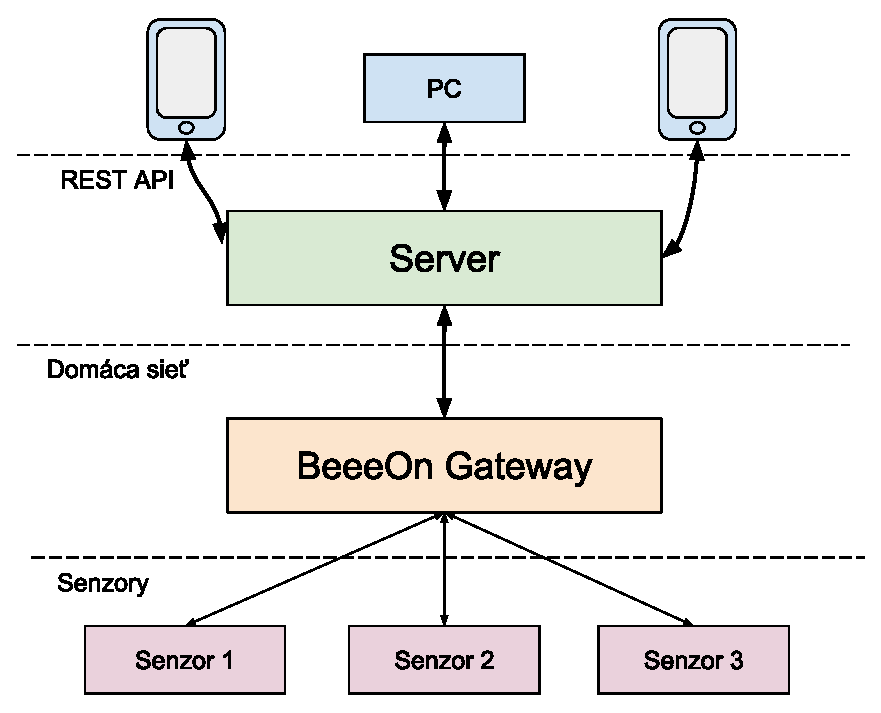
\includegraphics[width=220pt]{images/architektura.eps} 
	\caption{Architektúra systému BeeeOn}
	\label{architektura}
\end{figure}

Ako je vidno na obrázku \ref{architektura}, celý systém sa skladá z dvoch hlavných častí a to server a Gateway. Na najspodnejšej úrovni sú senzory, ktoré merajú dáta a následne ich posielajú komunikačným protokolom do Gateway aplikácie. Pre sprístupnenie niektorých komunikačných protokol je potrebné špeciálne USB zariadenie, ktoré na jednej strane komunikuje zo senzorom a na druhej strane s Gateway aplikáciou. Príkladom takýchto protokolov je IQRF, ZWave alebo Bluetooth. 

Gateway aplikácia môže byť spustená na ľubovoľnom systéme, ktorý podporuje potrebné knižnice pre preklad aplikácie. BeeeOn projekt pre túto aplikáciu používa open source hardware s vývojovou doskou A10-OLinuXino-LIME od spoločnosti Olimex. 

Po prijatí nameraných dát sa tieto dáta spracujú a prevedú do formátu, ktorý je spoločný pre všetky protokoly. Spracované dáta sa odošlú na server, kde sa tieto dáta uložia a je možné k ním pristupovať pomocou REST API.

\section{Testovacie prostredie}\label{testovacieProstredie}
Meraná lokalita je internátna izba, ktorá sa nachádza v meste Brno, v časti Královo pole. Budova, kde sa nachádza sledovaná miestnosť je v nezrekonštruovanom obytnom dome bez zateplenia s pôvodnými oknami. Izba je umiestnená na severovýchodnej strane a pred oknom je malý park. Objem miestnosti je približne $45\,m^3$. Počas všetkých meraní sa v miestnosti nachádzali maximálne tri osoby. 

V prípade vetrania sa mohlo okno nachádzať v dvoch polohách. Prvou polohou bolo plné otvorenie krídla a druhá poloha bolo otvorenie krídla o približne 20\,$^\circ$. Meranie prebiehalo dlhodobo a koncentrácia $CO_2$ sa merala každých 5\,s.

\section{Výber senzorov}
Systém BeeeOn podporuje dva druhy senzorov oxidu uhličitého, ktoré komunikujú bezdrôtovým protokolom IQRF. Pred začatím samotného merania bol zvolený jeden druh senzorov, aby namerané hodnoty neboli ovplyvnené rozdielnosťou senzorov. 

V tabuľke \ref{porovnanieCO2Senzorov} je možné vidieť vlastnosti jednotlivých senzorov od dvoch výrobcov, Protronix a IQ Home. Zo senzorov uvedených v tabuľke bol vybraný senzor od firmy Protronix, ktorý umožňuje napájanie externým zdrojom a má menší rozptyl hodnôt pri meraní koncentrácie $CO_2$ ako senzor od firmy IQ Home. Priebeh merania koncentrácie $CO_2$ oboch senzorov je zobrazený na obrázku \ref{imgIQHomeProtronix}. Pre orientačné meranie, kde nie je potrebná presnosť na desiatky ppm, by bol dostatočný aj senzor od firmy IQ Home.

Meranie bolo uskutočnené pri otvorení okna a nameraná hodnota sa posielala každých 15\,s, senzor bol umiestnený približne v strede miestnosti vo výške 60\,cm.

Na presnú detekciu otvorenia okna bol použitý senzor Jablotron JA-81M, ktorý bol umiestnený na okne a detekoval otvorenie alebo zatvorenie okna. Senzor posielal udalosti, v prípade, že sa okno otvorilo/zatvorilo a v prípade, že okno bolo otvorené tak posielal informáciu o tomto stave každých 9 minút.

\begin{table}[H]
\centering
\label{porovnanieCO2Senzorov}
\begin{tabular}{|c|l|l|}
\hline
\multicolumn{1}{|l|}{} & \multicolumn{1}{c|}{\textbf{\begin{tabular}[c]{@{}c@{}}Protronix\\ NLII-CO2+RH+T-IQRF\end{tabular}}} & \multicolumn{1}{c|}{\textbf{\begin{tabular}[c]{@{}c@{}}IQ Home\\ SN-THC-02\end{tabular}}} \\ \hline
\textbf{Podporované  veličiny} & $CO_2$, teplota, vlhkosť & CO2, teplota, vlhkosť \\ \hline
\textbf{$CO_2$ rozsah {[}ppm{]}} & 0--2000 (5000) & 0--5000 \\ \hline
\textbf{$CO_2$ presnosť} & $\pm \ 35\,ppm \ \pm \ 5\%$ z hodnoty & $\pm \ 50\,ppm \ \pm \ 3\%$ z hodnoty \\ \hline
\textbf{Druh napájania} & externým zdrojom & batériové napájanie \\ \hline
\end{tabular}
\caption{Parametre senzorov od firiem Protronix a IQ Home \cite{PorovnanieIQHome}, \cite{PorovnanieProtronix}}
\end{table}

\begin{figure}[H]
	\centering
	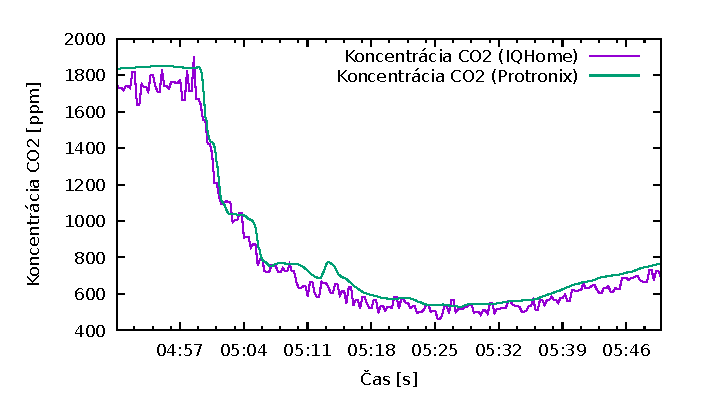
\includegraphics[width=430pt]{images/compareIqHomeProtronix.eps} 
	\caption{Nameraná koncentrácia $CO_2$ senzormi od firiem Protronix a IQ Home}
	\label{imgIQHomeProtronix}
\end{figure}

\section{Popis nameraných dát}
Po výbere senzorov bolo začaté meranie, ktoré prebiehalo na jednom mieste, ktoré je popísané v kapitole \ref{testovacieProstredie}. Meranie prebieha od 1.5.2018 do 3.6.2018 a na klasifikáciu je pripravených 78 hodnôt. Najvyššia nameraná koncentrácia bola $CO_2$ 2000\,ppm a najnižšia nameraná hodnota bola 328\,ppm. Hodnoty koncentrácie oxidu uhličitého sa merali každých 5\,s. Celkový počet dát je 543\,239 pre koncentráciu $CO_2$ a 2\,781 pre informácie o otvorení/zatvorení okna. Prístup k jednotlivým dátam je pomocou REST API, ktoré umožňuje stiahnutie nameraných údajov v určitých intervaloch.

Jednotlivé udalosti sú popísane v JSON súbore, ktorý obsahuje okrem času otvorenia a času zatvorenia aj doplnkové informácie o počte osôb v miestnosti, počasí vonku a polohe senzoru v miestnosti a na základe tohto súboru sa stiahnu potrebné informácie zo servera.

\chapter{Analýza nameraných dát}

\section{Weka}
Weka (Waikato Environment for Knowledge Analysis) je open source balík programov pre strojové učenie. Umožňuje modelovanie dát, ich analýzu a vizualizáciu. Pre Weku bol vytvorený vlastný textový formát ARFF (Attribute Relationship File Format), ktorý je podobný CSV súboru. Obsahuje atribúty, dodatočné informácie pre klasifikáciu a samotné dáta. Na začiatku súbora sú popísané jednotlivé stĺpce ich typy a rozsah ich hodnôt. Za popisom dát nasledujú jednotlivé dáta oddelené čiarkou. Weka podporuje rôzne druhy klasifikátorov. Klasifikátorom rozumieme problém určenia, do ktorej z kategórie dát nové pozorovanie patrí \cite{klasifikacia}. Weka podporuje niekoľko desiatok klasifikátorov a vrámci tejto práce boli vybrané štyri klasifikátory z rôznych kategórii na porovnanie\cite{wekaManual}:
\begin{itemize}
    \item ZeroR - Hľadanie dominantnej triedy, respektíve skupiny objektov s rovnakou charakteristikou.
    \item J48 - Rozhodovací strom, slúži na kategorizáciu atribútov.
    \item BayesNet - Bayesovská sieť využíva grafovú reprezentáciu pre zobrazenie pravdepodobností vzťahov medzi javmi.
    \item MultilayerPerceptron - Neurónová sieť, ktorá vytvára viacvrstvové grafy, do ktorých zanáša jednotlivé výskyty.
\end{itemize}

\section{Závislosť koncentrácie $CO_2$}\label{zavislostKoncentracie}
V teoretickej časti bolo spomenuté, že koncentrácia $CO_2$ závisí na počte osôb a ich činnosti. V tejto časti budú popísané namerané rozdiely medzi vyprodukovaným $CO_2$ pri rôznych činnostiach (v noci spánok, cez deň práca na počítači), pri rôznom počte osôb. Meranie prebiehalo v testovacom prostredí popísanom v kapitole \ref{testovacieProstredie}. 

\begin{figure}[H]
	\centering
	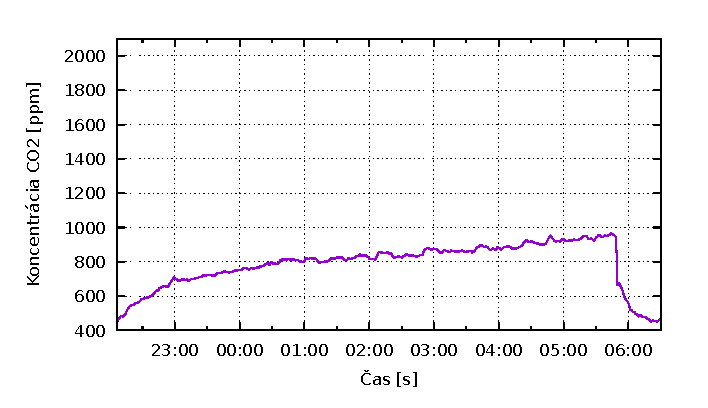
\includegraphics[width=350pt]{images/1clovekNocCO2.eps} 
	\caption{Koncentrácia $CO_2$ 1 osoby počas spánku}
	\label{img1osobaNoc}
\end{figure}
V grafe \ref{img1osobaNoc} je zobrazená produkcia $CO_2$ jednej osoby počas spánku. Pred začatím merania bola miestnosť vyvetraná na úroveň koncentrácia $CO_2$ vo vonkajšom prostredí. Po prebudení sa vykonala obdobná akcia. Meranie prebiehalo medzi 2.6.2018 22:06 a 3.6.2018 07:30. Maximálna úroveň koncentrácie $CO_2$ bola 965\,ppm a bola dosiahnutá 4.6.2018 05:43. V grafe je vidno približne rovnaký prírastok $CO_2$ počas celej doby spánku okrem začiatku a konca merania. Pri konci merania je to spôsobené otvorením okna v čase 05:45. Priemerný hodinový prírastok $CO_2$ je približne 40\,ppm (meraný od 00:00--05:45).

\begin{figure}[H]
	\centering
	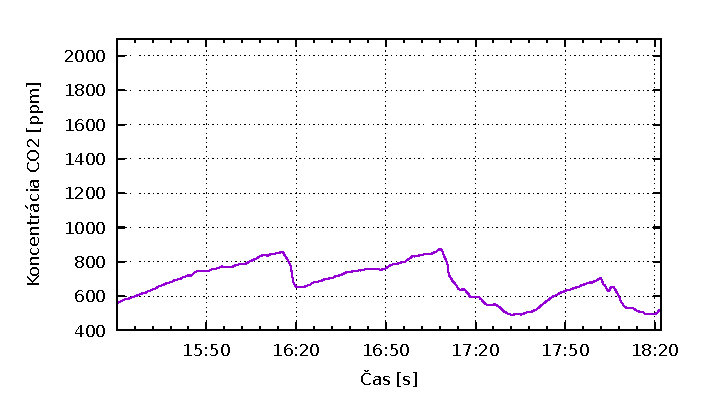
\includegraphics[width=350pt]{images/1clovekDennaAktivitaCO2.eps} 
	\caption{Koncentrácia $CO_2$ 1 osoby vo vybraný čas dňa počas práce na počítači}
	\label{img1osobaDen}
\end{figure}
V grafe \ref{img1osobaDen} je zobrazená produkcia $CO_2$ jednej osoby počas práce na počítači. Práca na počítači vyžaduje viacej energie ako spánok. Pred začatím  merania bola miestnosť vyvetraná, aby sa dosiahla koncentrácia $CO_2$ vo vonkajšom prostredí. Strmí pokles koncentrácie v grafe znázorňuje vetranie v priebehu práce na počítači. Meranie prebiehalo medzi 12.5.2018 15:20 a 12.5.2018 18:22. Maximálna úroveň koncentrácie bola 874\,ppm v čase 17:08. V grafe je vidno približne rovnaký prírastok $CO_2$, až na čas, kedy bolo otvorené okno. Priemerný prírastok $CO_2$ pri zatvorenom okne je približne 140\,ppm za hodinu, pričom dĺžka jednotlivých vetraní bola: 5 minút, 27 minút a 18 minút.

\begin{figure}[H]
	\centering
	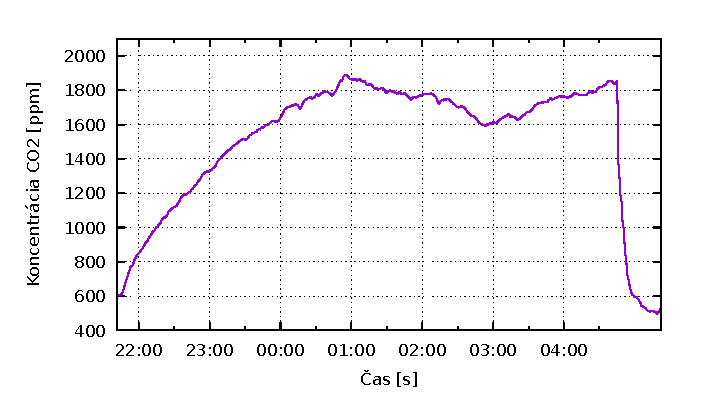
\includegraphics[width=350pt]{images/2ludiaNocCO2.eps} 
	\caption{Koncentrácia $CO_2$ 2 osôb počas spánku}
	\label{img2osobyNoc}
\end{figure}
V grafe \ref{img2osobyNoc} je zobrazená produkcia $CO_2$ dvoch osôb počas spánku. Pre začatím merania bola miestnosť vyvetraná na úroveň koncentrácie $CO_2$ vo vonkajšom prostredí. Po prebudení sa vykonala podobná akcia. Meranie prebiehalo medzi 1.5.2018 21:41 a 2.5.2018 05:22. Maximálna úroveň koncentrácie $CO_2$ bola 1887\,ppm v čase 1.5.2018 00:55. V grafe je vidno 3 úseky spánku, ktoré sa dajú rozdeliť na základe hodinového prírastku koncentrácie $CO_2$. Prvých 200 minút bol hodinový prírastok približne 390\,ppm, ďalšie dve hodiny bol hodinový prírastok približne $-150$\,ppm a ďalšie 2 hodiny bol hodinový prírastok približne 125\,ppm. Zmeny prírastku $CO_2$ sú spôsobené rôznymi fázami spánku.

\begin{figure}[H]
	\centering
	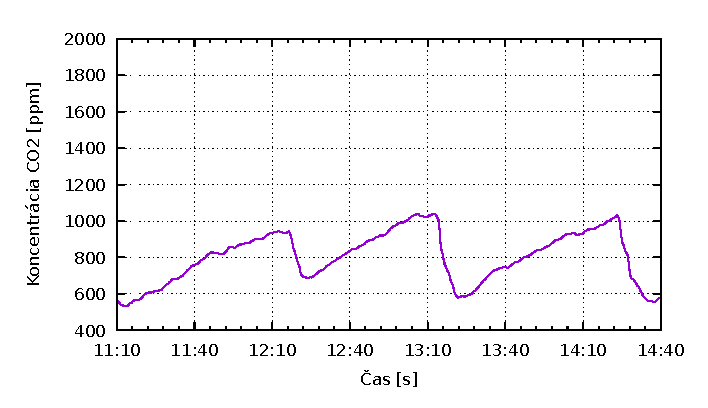
\includegraphics[width=350pt]{images/2ludiaDennaAktivitaCO2.eps} 
	\caption{Koncentrácia $CO_2$ 2 osôb vo vybraný čas dňa počas práce na počítači}
	\label{img2osobyDen}
\end{figure}
Posledný \ref{img2osobyDen} graf popisuje produkciu $CO_2$ dvoch osôb počas práce na počítači. Práca na počítači vyžaduje viacej energie ako spánok. Pred začatím merania prebehlo vetrania, aby sa dosiahla koncentrácia $CO_2$ vo vonkajšom prostredí. Strmí pokles koncentrácie v grafe znázorňuje vetranie v priebehu práce na počítači. Meranie prebehlo medzi 5.5.2018 11:10 a 5.5.2018 14:40. maximálna úroveň koncentrácie bola 1040\,ppm v čase 15:06. V grafe je vidieť približne rovnaký hodinový prírastok 210\,ppm, pričom dĺžka jednotlivých vetraní bola: 5 minút, 8 minút a 11 minút.
\\\\
Pre zistenie vonkajšej koncentrácie $CO_2$ prebehlo meranie po dobu 24 hodín v čase 1.6.2018 10:00--2.6.2018 10:00. V túto dobu bol umiestnený senzor na vonkajšej parapete okna a meral koncentráciu $CO_2$ vonku. Priemerná koncentrácia $CO_2$ za 24 hodín v meranom mieste bola 434\,ppm.

\begin{figure}[H]
	\centering
	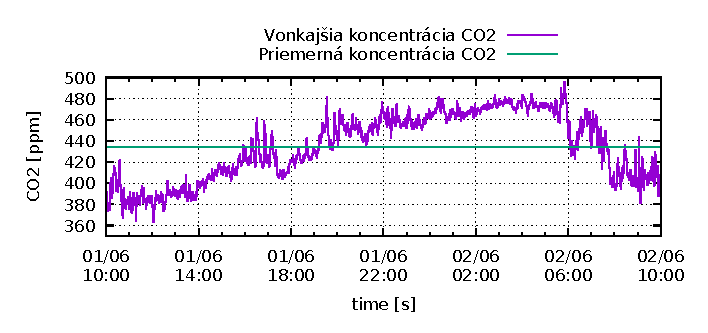
\includegraphics[width=420pt]{images/vonkajsieCO2-24h.eps} 
	\caption{Koncentrácia vonkajšieho vzduchu $CO_2$}
	\label{imgPriemernaKoncentracia}
\end{figure}


\section{Výber atribútov a voľba vhodného klasifikátora pre detekciu otvorenia okna}\label{sectionOtvoreniOkna}
Pred samotnou klasifikáciou v programe Weka, je potrebné vytvoriť ARFF súbor s potrebnými atribútmi podľa, ktorých sa môže klasifikovať otvorenie okna. Z obrázku \ref{imgOtvorenieOkna} je vidieť, že samotné akcie otvorenia alebo zatvorenia okna nám neprinášajú žiadne informácie, dokonca ani hodnoty, ktoré sú vo veľmi tesnej blízkosti, pretože po otvorení okna bolo potrebných až 90\,s pokiaľ sa koncentrácia $CO_2$ začala znižovať.

V prípade, že by sme zvolili ako atribúty samotné hodnoty koncentrácie $CO_2$, klasifikátor by sa naučil len presné rozsahy, ktoré by boli obsiahnuté v trénovacej množine. Problémy by nastali pri overení na inej množine dát, kde by mohlo prísť k intenzívnejšiemu alebo menej intenzívnejšiemu poklese koncentrácie $CO_2$ ako v trénovacej množine, čo by spôsobilo nesprávne klasifikovanie hodnôt, rozsah hodnôt by bol daný inak.

\begin{figure}[H]
	\centering
	\includegraphics[width=350pt]{images/vyberParametrov.eps} 
	\caption{Typický pokles koncentrácie $CO_2$ pri otvorení okna}
	\label{imgOtvorenieOkna}
\end{figure}

Ako atribúty boli teda zvolené derivácia, ktoré určia podľa svojho znamienka, či koncentrácia klesá alebo rastie a podľa veľkosti hodnoty nám dájú informáciu ako veľmi rastie alebo klesá. V obrázkoch z kapitoly \ref{zavislostKoncentracie} a obrázku \ref{imgOtvorenieOkna}, je vidno, že derivácie, by nám správne určili znamienkom pokles a hodnotou veľkosť poklesu koncentrácie $CO_2$.

%derivacie: nabeh, rychlost

Pred začatím testovania klasifikátorov, bolo potrebné ešte vyriešiť problém kedy učenie prebieha na množine dát, ktorá je rozdelená do dvoch tried s približne rovnakým počtom. V našom prípade jedna trieda obsahuje informácie o tom, že otvorenie okno nastalo a druhá trieda o tom, že daná udalosť nenastala. Údaje o tom, že daná udalosť nenastala boli získané tak, že od času, kedy nastalo otvorenie okna sme sa posunuli o stanovený čas dozadu. V tomto čase sme predpokladali, že okno nebolo otvorené a derivácie sa vypočítali rovnakým spôsobom ako pre otvorenie okna.

\begin{table}[H]
\centering
\begin{tabular}{|c|c|c|c|c|c|c|c|c|c|c|}
\hline
\multirow{2}{*}{\textbf{\begin{tabular}[c]{@{}c@{}}\end{tabular}}} & \multicolumn{10}{c|}{\textbf{Interval opakovania derivácie}} \\ \cline{2-11} 
 & \textbf{10} & \textbf{20} & \textbf{30} & \textbf{40} & \textbf{50} & \textbf{60} & \textbf{70} & \textbf{80} & \textbf{90} & \textbf{100} \\ \hline
\textbf{\begin{tabular}[c]{@{}c@{}}Neurónová\\ sieť\end{tabular}} & 47.4 & 50.0 & 76.3 & 81.6 & 80.3 & 80.3 & 75.0 & 81.6 & 81.6 & 69.7 \\ \hline
\textbf{J48} & 39.4 & 61.8 & 79.0 & 81.6 & 88.2 & 88.2 & 82.9 & 82.9 & 79.0 & 64.5 \\ \hline
\textbf{ZeroR} & 47.4 & 47.4 & 47.4 & 47.4 & 47.4 & 47.4 & 47.4 & 47.4 & 47.4 & 47.4 \\ \hline
\textbf{\begin{tabular}[c]{@{}c@{}}Bayesovská\\ sieť\end{tabular}} & 47.4 & 56.6 & 77.6 & 81.6 & 80.3 & 80.3 & 88.2 & 88.2 & 73.7 & 72.4 \\ \hline
\textbf{Priemer} & \textbf{45.4} & \textbf{54.0} & \textbf{70.1} & \textbf{73.1} & \textbf{74.1} & \textbf{74.1} & \textbf{73.4} & \textbf{75.1} & \textbf{70.4} & \textbf{63.5} \\ \hline
\end{tabular}
\label{tab1}
\caption{Úspešnosť klasifikátorov s rozličnými intervalmi opakovania derivácií}
\end{table}

Tabuľka \ref{tab1} zobrazuje rôzne intervaly derivácií. Interval derivácií môžeme chápať ako čas po, ktorom sa vytvori derivácia a použije sa na klasifikáciu. Pri tomto testovaní sa použili 3 derivácie a čas udalosti kedy nebolo okno otvorené, bol nastavený na 100\,s dozadu. Z tabuľky je vidno, že interval derivácií 40--80 poskytoval najlepšie výsledky.

\begin{table}[H]
\centering
\begin{tabular}{|c|c|c|c|c|c|c|}
\hline
\multirow{2}{*}{\textbf{\begin{tabular}[c]{@{}c@{}}Typ\\ Klasifikátora\end{tabular}}} & \multicolumn{6}{c|}{\textbf{Počet derivácií}} \\ \cline{2-7} 
 & \textbf{1} & \textbf{2} & \textbf{3} & \textbf{4} & \textbf{5} & \textbf{6} \\ \hline
\textbf{\begin{tabular}[c]{@{}c@{}}Neurónová\\ sieť\end{tabular}} & 44.7 & 76.3 & 82.9 & 80.3 & 84.2 & 73.7 \\ \hline
\textbf{J48} & 43.4 & 69.7 & 89.5 & 88.2 & 88.2 & 88.2 \\ \hline
\textbf{ZeroR} & 47.4 & 47.4 & 47.4 & 47.4 & 47.4 & 47.4 \\ \hline
\textbf{\begin{tabular}[c]{@{}c@{}}Bayesovská\\ sieť\end{tabular}} & 47.4 & 72.4 & 82.9 & 80.3 & 81.6 & 80.3 \\ \hline
\textbf{Primer} & \multicolumn{1}{l|}{\textbf{46.6}} & \multicolumn{1}{l|}{\textbf{66.5}} & \multicolumn{1}{l|}{\textbf{75.7}} & \multicolumn{1}{l|}{\textbf{74.1}} & \multicolumn{1}{l|}{\textbf{75.1}} & \multicolumn{1}{l|}{\textbf{72.4}} \\ \hline
\end{tabular}
\label{tab2}
\caption{Úspešnosť klasifikátorov v závislosti od počtu derivácií}
\end{table}

Tabuľka \ref{tab2} popisuje rôzny počet derivácií. Počet derivácií môžeme chápať ako počet atribútov pre klasifikovanie. Pri testovaní sa použil interval derivácií 50\,s a čas udalosti kedy nebolo okno otvorené, bol nastavený na 100\,s dozadu. Z tabuľky je vidno, že najlepší počet derivácií je 3--5.

\begin{table}[H]
\centering
\begin{tabular}{|c|c|l|l|l|l|l|l|l|l|l|l|}
\hline
\multirow{2}{*}{\textbf{}} & \multicolumn{11}{c|}{\textbf{Čas udalosti, kedy nebolo okno otvorené}} \\ \cline{2-12} 
 & \textbf{90} & \textbf{105} & \textbf{120} & \textbf{135} & \textbf{160} & \textbf{175} & \textbf{190} & \textbf{205} & \textbf{220} & \textbf{235} & \textbf{250} \\ \hline
\textbf{\begin{tabular}[c]{@{}c@{}}Neurónová\\ sieť\end{tabular}} & 78.9 & 77.6 & 75.0 & 86.8 & 65.8 & 77.6 & 86.8 & 84.2 & 86.8 & 82.9 & 82.9 \\ \hline
\textbf{J48} & 76.3 & 85.5 & 82.9 & 88.2 & 88.2 & 93.4 & 90.8 & 90.8 & 88.2 & 84.2 & 84.2 \\ \hline
\textbf{ZeroR} & 47.4 & 47.4 & 47.4 & 47.4 & 47.4 & 47.4 & 47.4 & 47.4 & 47.4 & 47.4 & 47.4 \\ \hline
\textbf{\begin{tabular}[c]{@{}c@{}}Bayesovská\\ sieť\end{tabular}} & 81.6 & 86.8 & 85.5 & 88.2 & 78.9 & 89.4 & 89.5 & 90.8 & 88.2 & 84.2 & 84.2 \\ \hline
\textbf{Priemer} & \multicolumn{1}{l|}{\textbf{71.1}} & \textbf{74.3} & \textbf{72.7} & \textbf{77.7} & \textbf{72.4} & \textbf{77.0} & \textbf{78.6} & \textbf{78.3} & \textbf{77.7} & \textbf{74.7} & \textbf{74.7} \\ \hline
\end{tabular}
\caption{Úspešnosť klasifikátorov v závislosti od času udalosti, kedy nedošlo k otvoreniu}
\label{tab3}
\end{table}

Tabuľka \ref{tab3} znázorňuje rôzny čas udalosti, kedy nebolo okno otvorené. Tento údaj slúži na vygenerovanie záznamu pre strojové učenie, aby bol počet záznamov, ktoré sú a nie sú udalosťou rovnaký. Pri testovaní sa použil interval derivácií 50\,s a počet derivácií 3. Z tabuľky je vidno, že najlepší čas, kedy nebolo okno otvorené je v rozsahu 175--220.
\\\\
Ako výsledný klasifikátor bol zvolený J48, ktorý dosahoval v experimentoch veľmi dobré výsledky. Rozhodovací strom je názorný a jeho implementácia je priamočiara. Pre výsledný klasifikátor boli zvolená nasledujúce parametre:
\begin{itemize}
    \item interval opakovania derivácií: $50 \in \{40, 50, 60, 70, 80\{$
    \item počet derivácií: $3 \in \{3, 4, 5\}$
    \item čas udalosti, kedy nebolo okno otvorené: $175 \in \{175, 190, 205, 220\}$
\end{itemize}

\noindent Na zhodnotenie kvality klasifikátora bola použitá ROC krivka, ktorú je možné vidieť na obrázku \ref{imgRocKrivka}. Plocha pod ROC krivkou má hodnotu: 0.9072.

\begin{figure}[H]
	\centering
	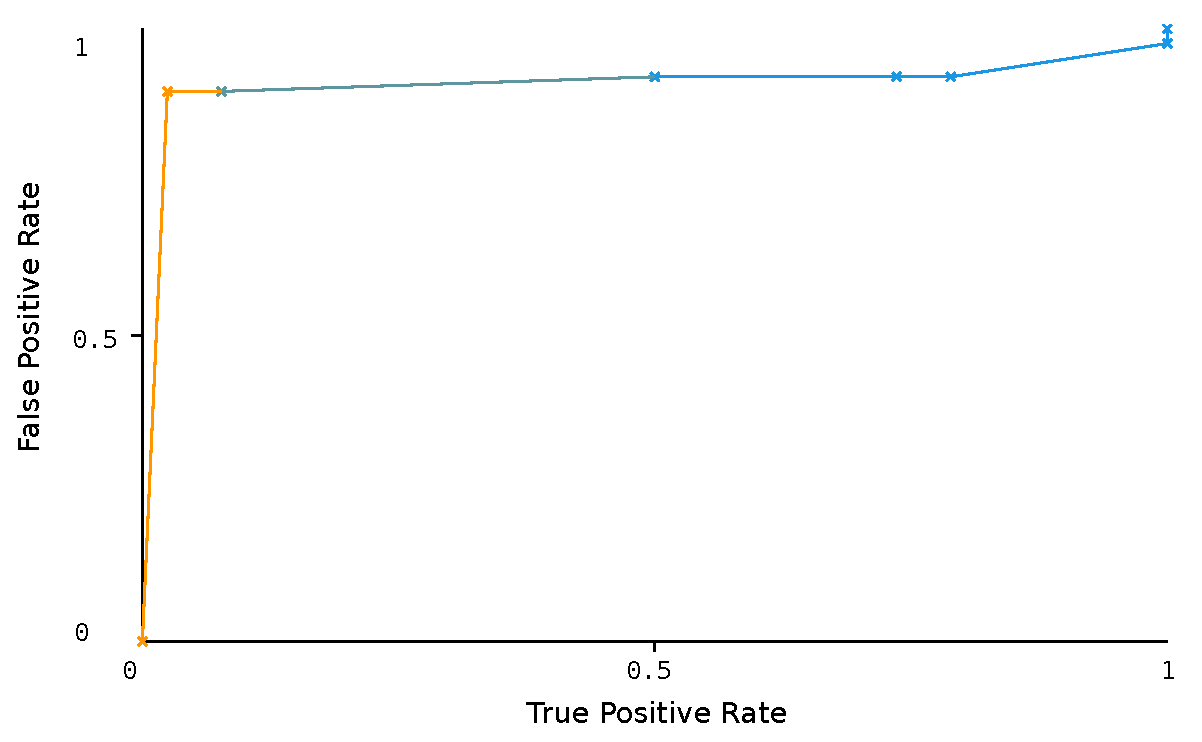
\includegraphics[width=320pt]{images/roc.eps} 
	\caption{ROC krivka hodnotiaca J48 klasifikátor}
	\label{imgRocKrivka}
\end{figure}

\chapter{Záver}
Cieľom práce bolo vybrať vhodné senzory na meranie oxidu uhličitého vo vnútri budov a na základe vykonaných meraní stanoviť závislosť koncentrácie oxidu uhličitého na nameraných veličinách. Na základe stanovenej závislosti vytvoriť atribúty pre strojové učenie a vytvoriť model pre detekciu otvorenia okna.

V práci bola naštudovaná problematika merania kvality ovzdušia, ktorá sa merania koncentráciou oxidu uhličitého. Koncentráciu $CO_2$ vo vnútri budov najviac ovplyvňujú ľudia a množstvo vymieňaného vzduchu (intenzita vetrania). V texte boli popísané vlastnosti $CO_2$ a jeho účinky pri vyšších koncentráciách, ktoré môžu spôsobovať únavu, bolesti hlavy a hrdla. Čím je vykonávaná väčšia fyzická aktivita, tým sa koncentrácia $CO_2$ zvyšuje rýchlejšie.

Pred začiatkom meraní bolo potrebné naštudovať architektúru BeeeOn a vybrať vhodné senzory na meranie a následne ich prepojiť s týmto meraním a začať merať. Pre meranie boli vybrané senzory od firmy Protronix, ktoré majú menšie odchýlky a umožňujú byť napájané externým zdrojom. Tabuľkové hodnoty presnosti oboch senzorov boli odmerané a vynesené do obrázku \ref{imgIQHomeProtronix}.

V praktickej časti boli namerané závislosti koncentrácie $CO_2$ medzi počtom osôb a vykonávanou aktivitou. Pri spánku jednej osoby je priemerný hodinový prírastok $CO_2$ približne 40\,ppm v miestnosti s objemom $45m^3$ a pri kancelárskej práci je tento hodinový prírastok približne 150\,ppm. Ak sa jedná o 2 osoby hodinový prírastok počas spánku závisel od fáze spánku. Prvých 200 minút bol hodinový prírastok 150\,ppm, ďalšie 2 hodiny $-150$\,ppm a ďalšie 2 hodiny 125\,ppm. V prípade kancelárskej práce je hodinový prírastok 2 osôb na úrovni 210\,ppm.

Z nameraných dát boli použité derivácie ako atribút pre klasifikovanie. Dôvodom bolo, že pri otvorení okna koncentrácia $CO_2$ prudko poklesne a táto skutočnosť je dobre reprezentovaná deriváciami. 

Na základe zistených závislosti sa vytvorili klasifikátory otvorenia okna, kde sa v kapitole \ref{sectionOtvoreniOkna} experimentálne zistilo, že klasifikátory pracujú ideálne s intervalom opakovania derivácie: 40, 50, 70, 80, s počtom derivácií: 3,4,5 a časom udalosti, kedy nebolo okno otvorené: 175, 190, 205, 220.

Ako klasifikátor pre detekciu otvorenia okna bol zvolený klasifikátor J48 s parametrami opakovania derivácie 50, s počtom derivácií 3 a časom udalosti, kedy nebolo okno otvorené 175. Klasifikátor bol ohodnotení pomocou ROC krivky, kde plocha pod krivkou je 0.9072, čo začí o veľmi kvalitnom klasifikátore.




% https://www.wikiskripta.eu/w/ROC_křivka
% vyhodnotenie klasifikatora


% derivacie: rychlost, nabeh


%do DP:
% rozsirit teoriu o podrobnejsi popis klasifikatorov a weky cca 5stran
% vytvorit nejaky model CO2, pekne spracovane je to v DP: Modelování a řízení obsahu CO2.pdf a v clanku http://www.istavebnictvo.sk/clanky/vydychany-vzduch-a-ako-ho-spravne-vyvetrat/

% idelane by bolo upravit grafy pre analyzovanie koncentracie CO2,
% pocet osob: 1,2,3
% aktivita: spanok, praca u pc
% dat ich do jedneho grafu a snazit sa to odmerat v rovnaky cas, pripadne to nejak vymysliet.

% popisat ROC krivku